\documentclass{beamer}
\usepackage{fancyvrb}
\usepackage{hyperref}
\usepackage{multicol}
\usepackage{graphicx}
\usepackage{xcolor}
\newtheorem{theo}{Theorem}[section]

\newcommand{\myfig}[1]{\centerline{\includegraphics[scale=0.25]{figures/#1.png}}}

\newcommand{\trans}[5]{
\begin{tabular}{|c|c|c|c|c|}\hline
#1 & #2 & #3 & #4 & #5 \\\hline
\end{tabular}
}

\newcommand{\arr}{&\rightarrow&}
\newcommand{\darr}{&\Rightarrow&}
\newcommand{\ar}{\rightarrow}
\newcommand{\dar}{\Rightarrow}
\newcommand{\bee}{\begin{eqnarray*}}
\newcommand{\eee}{\end{eqnarray*}}
\newcommand{\lmb}{\ensuremath{\lambda}}

\newcommand{\bi}{\begin{itemize}}
\newcommand{\ii}{\item}
\newcommand{\ei}{\end{itemize}}

\newcommand{\sect}[1]{
\section{#1}
\begin{frame}[fragile]\frametitle{#1}
}

\mode<presentation>
{
%  \usetheme{Madrid}
  % or ...

%  \setbeamercovered{transparent}
  % or whatever (possibly just delete it)
}

\usepackage[english]{babel}

\usepackage[latin1]{inputenc}

\title
{
Scheme Notes 04
}

\subtitle{
} % (optional)

\author[Geoffrey Matthews]
{Geoffrey Matthews}
% - Use the \inst{?} command only if the authors have different
%   affiliation.

\institute[WWU/CS]
{
  Department of Computer Science\\
  Western Washington University
}
% - Use the \inst command only if there are several affiliations.
% - Keep it simple, no one is interested in your street address.

\date{\today}

% If you have a file called "university-logo-filename.xxx", where xxx
% is a graphic format that can be processed by latex or pdflatex,
% resp., then you can add a logo as follows:

%\pgfdeclareimage[height=0.5cm]{university-logo}{WWULogoProColor}
%\logo{\pgfuseimage{university-logo}}

% If you wish to uncover everything in a step-wise fashion, uncomment
% the following command: 

%\beamerdefaultoverlayspecification{<+->}

\begin{document}

\begin{frame}
  \titlepage
\end{frame}


\newcommand{\myref}[1]{\small\item\url{#1}}
\newcommand{\myreft}[1]{\footnotesize\item\url{#1}}

%\begin{frame}
%  \frametitle{Outline}
%  \tableofcontents
%  % You might wish to add the option [pausesections]
%\end{frame}

\sect{Trees}

\begin{Verbatim}
(define tree1 (cons (list 1 2) (list 3 4)))

(define tree2 (list (list 1 2)
                    (list 3
                          (list 4 5 6))
                    (list 7 8)))
\end{Verbatim}

\begin{itemize}
\item Run {\tt boxarrow.rkt} for pictures.
\end{itemize}
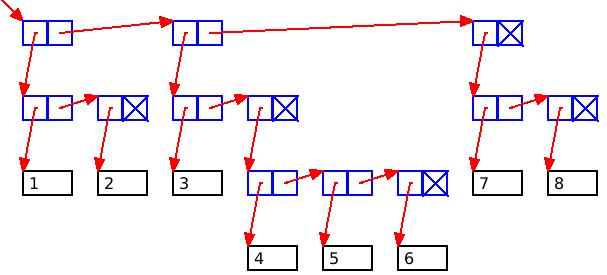
\includegraphics[width=\textwidth]{tree}
\end{frame}
\sect{count-leaves}
\pause
\begin{Verbatim}
(define (count-leaves tree)
  (cond ((empty? tree) 0)
        ((not (pair? tree)) 1)
        (else (+ (count-leaves (car tree))
                 (count-leaves (cdr tree))))))
\end{Verbatim}
\end{frame}
\sect{fringe}
\pause
\begin{Verbatim}
(define (fringe tree)
  (cond ((empty? tree) '())
        ((not (pair? tree)) (list tree))
        (else (append (fringe (car tree))
                      (fringe (cdr tree))))))
\end{Verbatim}
\end{frame}
\sect{sum-fringe}
\pause
\begin{Verbatim}
(define (sum-fringe tree)
  (cond ((empty? tree) 0)
        ((number? tree) tree)
        (else (+ (sum-fringe (car tree))
                 (sum-fringe (cdr tree))))))
\end{Verbatim}
\end{frame}
\sect{map-tree}
\pause
\begin{Verbatim}
(define (map-tree tree op)
  (cond ((empty? tree) '())
        ((not (pair? tree)) (op tree))
        (else (cons (map-tree (car tree) op)
                    (map-tree (cdr tree) op)))))
\end{Verbatim}
\end{frame}
\sect{scale-tree using map-tree}
\pause
\begin{Verbatim}
(define (scale-tree tree factor)
  (map-tree tree (lambda (x) (* x factor))))
\end{Verbatim}
\end{frame}
\sect{increment-tree using map-tree}
\pause
\begin{Verbatim}
(define (increment-tree tree)
  (map-tree tree inc))
\end{Verbatim}

\end{frame}


\sect{Apply}

\begin{Verbatim}
  (+ 1 2 3 4 5)               =>  15
  (+ (list 1 2 3 4 5))        =>  error 
  (apply + (list 1 2 3 4 5))  =>  15
\end{Verbatim}

\end{frame}
\end{document}
